\documentclass[11pt]{article}

\usepackage[a4paper,margin=1in]{geometry}
\usepackage{amsmath,amssymb}
\usepackage{booktabs}
\usepackage{array}
\usepackage{graphicx}
\usepackage{float}
\usepackage{hyperref}
\usepackage{tikz}
\usepackage{xcolor}
\usetikzlibrary{arrows.meta,positioning,calc,fit}

\hypersetup{
  colorlinks=true,
  linkcolor=blue!45!black,
  urlcolor=blue!45!black,
  citecolor=blue!45!black
}

\title{ARIA-GOLF v1--v5: Structural Differences and Model Equations}
\author{Internal architecture note}
\date{\today}

\newcommand{\fs}{f_{\mathrm{s}}}
\newcommand{\src}{s}
\newcommand{\harm}{h}
\newcommand{\noise}{\eta}
\newcommand{\vt}{H_{\mathrm{VT}}}
\newcommand{\room}{H_{\mathrm{room}}}
\newcommand{\nfilt}{H_{\mathrm{N}}}
\newcommand{\ap}{A}
\newcommand{\lf}{g_{\mathrm{LF}}}
\newcommand{\biquad}{B}
\newcommand{\pole}{P}
\newcolumntype{L}[1]{>{\raggedright\arraybackslash}p{#1}}

\begin{document}
\maketitle

\begin{abstract}
This note reorganizes the v1--v5 ARIA-GOLF configuration differences into a
model-comparison form. All versions share the same encoder family, observed
F0 conditioning, LF glottal-flow oscillator, white-noise generator, room
filter, and multi-scale spectrogram loss. The relevant architectural
differences are localized to two places: the analytic vocal-tract cascade
(v1--v3) and the harmonic/noise excitation topology (v3--v5). In all versions,
the harmonic and noise branches are first combined into one source signal
$\src$, and this combined source is then passed through the vocal tract once.
The equations below make these changes explicit so that the five variants can
be presented as an interpretable ablation sequence.
\end{abstract}

\section*{How to Read the Five Versions}

The simplest reading is that v1--v3 are not five unrelated systems. They are
an ablation path with two axes. First, v1--v3 refine the analytic vocal tract:
the model searches for a useful balance between explicit formant control,
bandwidth constraints, spectral tilt, and learned residual all-pole capacity.
Second, v4 and v5 keep the v3 vocal tract and change only the excitation
mixture, because the remaining artifact is caused by additive harmonic-plus-noise
synthesis.

\begin{figure}[ht]
\centering
\resizebox{\linewidth}{!}{%
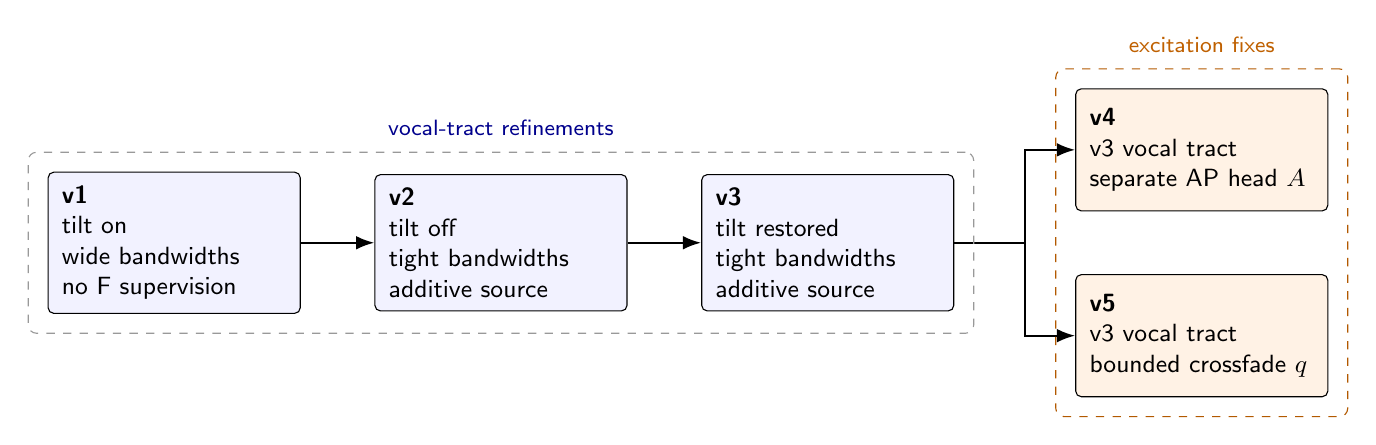
\begin{tikzpicture}[
  font=\sffamily\small,
  >=Latex,
  model/.style={draw=black, rounded corners=2pt, align=left, text width=2.85cm,
    minimum height=1.55cm, inner sep=5pt, fill=white},
  vt/.style={model, fill=blue!5},
  src/.style={model, fill=orange!10},
  band/.style={draw=black!40, dashed, rounded corners=3pt, inner sep=7pt},
  note/.style={align=center, font=\sffamily\footnotesize},
  arrow/.style={->, line width=0.8pt}
]
  \node[vt] (v1) at (0,0) {\textbf{v1}\\tilt on\\wide bandwidths\\no F supervision};
  \node[vt] (v2) at (4.15,0) {\textbf{v2}\\tilt off\\tight bandwidths\\additive source};
  \node[vt] (v3) at (8.3,0) {\textbf{v3}\\tilt restored\\tight bandwidths\\additive source};
  \node[src] (v4) at (13.05,1.18) {\textbf{v4}\\v3 vocal tract\\separate AP head $A$};
  \node[src] (v5) at (13.05,-1.18) {\textbf{v5}\\v3 vocal tract\\bounded crossfade $q$};

  \draw[arrow] (v1) -- (v2);
  \draw[arrow] (v2) -- (v3);
  \coordinate (split) at ($(v3.east)+(0.9,0)$);
  \draw[arrow] (v3.east) -- (split) |- (v4.west);
  \draw[arrow] (v3.east) -- (split) |- (v5.west);
  \node[band, fit=(v1)(v2)(v3)] (vtband) {};
  \node[band, draw=orange!70!black, fit=(v4)(v5)] (srcband) {};
  \node[note, blue!55!black, above=0.08cm of vtband] {vocal-tract refinements};
  \node[note, orange!75!black, above=0.08cm of srcband] {excitation fixes};
\end{tikzpicture}}
\vspace{2pt}

{\footnotesize v1$\rightarrow$v2: tighten F/B ranges \qquad
v2$\rightarrow$v3: restore spectral tilt}
\caption{Conceptual lineage of ARIA-GOLF v1--v5. v1--v3 should be read as
vocal-tract refinements; v4 and v5 are two alternative fixes for the same
high-band excitation artifact. v1 is also the unsupervised-formant baseline.}
\label{fig:lineage}
\end{figure}

\begin{figure}[ht]
\centering
\resizebox{\linewidth}{!}{%
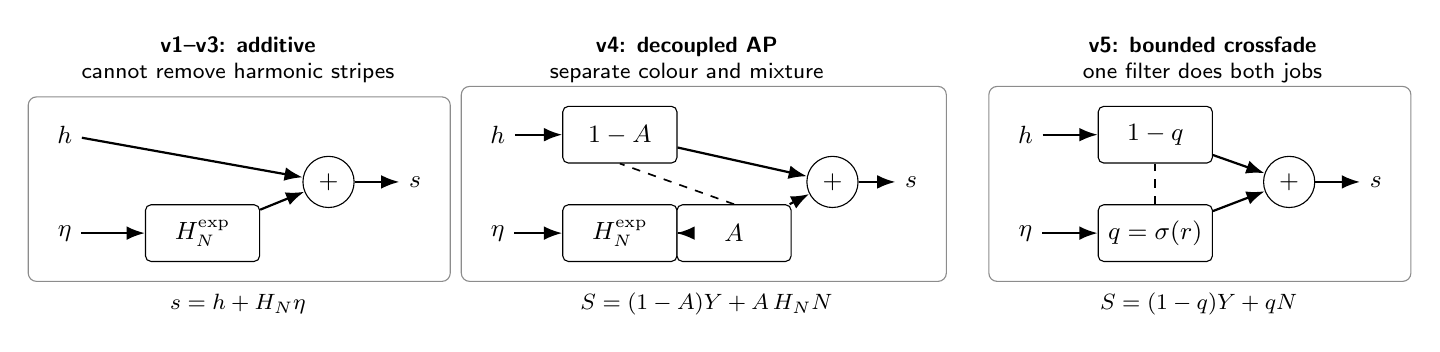
\begin{tikzpicture}[
  font=\sffamily\small,
  >=Latex,
  block/.style={draw=black, rounded corners=2pt, align=center,
    minimum width=1.45cm, minimum height=0.72cm, inner sep=3pt, fill=white},
  sum/.style={draw=black, circle, align=center, minimum size=0.65cm, inner sep=0pt, fill=white},
  panel/.style={draw=black!45, rounded corners=3pt, inner sep=7pt},
  flow/.style={->, line width=0.8pt},
  lbl/.style={font=\sffamily\footnotesize, align=center}
]
  % v1-v3 additive
  \begin{scope}[xshift=0cm]
    \node[lbl] at (2.2,2.2) {\textbf{v1--v3: additive}\\cannot remove harmonic stripes};
    \node (h1) at (0,1.25) {$h$};
    \node (n1) at (0,0) {$\eta$};
    \node[block] (hn1) at (1.75,0) {$H_N^{\exp}$};
    \node[sum] (sum1) at (3.35,0.65) {$+$};
    \node (s1) at (4.45,0.65) {$s$};
    \draw[flow] (h1) -- (sum1);
    \draw[flow] (n1) -- (hn1);
    \draw[flow] (hn1) -- (sum1);
    \draw[flow] (sum1) -- (s1);
    \node[lbl] at (2.2,-0.9) {$s=h+H_N\eta$};
    \node[panel, fit=(h1)(n1)(hn1)(sum1)(s1)] {};
  \end{scope}

  % v4 decoupled
  \begin{scope}[xshift=5.5cm]
    \node[lbl] at (2.4,2.2) {\textbf{v4: decoupled AP}\\separate colour and mixture};
    \node (h2) at (0,1.25) {$h$};
    \node (n2) at (0,0) {$\eta$};
    \node[block] (onea) at (1.55,1.25) {$1-A$};
    \node[block] (hn2) at (1.55,0) {$H_N^{\exp}$};
    \node[block] (a2) at (3.0,0) {$A$};
    \node[sum] (sum2) at (4.25,0.65) {$+$};
    \node (s2) at (5.25,0.65) {$s$};
    \draw[flow] (h2) -- (onea);
    \draw[flow] (onea) -- (sum2);
    \draw[flow] (n2) -- (hn2);
    \draw[flow] (hn2) -- (a2);
    \draw[flow] (a2) -- (sum2);
    \draw[flow] (sum2) -- (s2);
    \draw[dashed, line width=0.6pt] (a2.north) -- (onea.south);
    \node[lbl] at (2.65,-0.9) {$S=(1-A)Y+A\,H_NN$};
    \node[panel, fit=(h2)(n2)(onea)(hn2)(a2)(sum2)(s2)] {};
  \end{scope}

  % v5 bounded crossfade
  \begin{scope}[xshift=12.2cm]
    \node[lbl] at (2.25,2.2) {\textbf{v5: bounded crossfade}\\one filter does both jobs};
    \node (h3) at (0,1.25) {$h$};
    \node (n3) at (0,0) {$\eta$};
    \node[block] (oneq) at (1.65,1.25) {$1-q$};
    \node[block] (q3) at (1.65,0) {$q=\sigma(r)$};
    \node[sum] (sum3) at (3.35,0.65) {$+$};
    \node (s3) at (4.45,0.65) {$s$};
    \draw[flow] (h3) -- (oneq);
    \draw[flow] (oneq) -- (sum3);
    \draw[flow] (n3) -- (q3);
    \draw[flow] (q3) -- (sum3);
    \draw[flow] (sum3) -- (s3);
    \draw[dashed, line width=0.6pt] (q3.north) -- (oneq.south);
    \node[lbl] at (2.2,-0.9) {$S=(1-q)Y+qN$};
    \node[panel, fit=(h3)(n3)(oneq)(q3)(sum3)(s3)] {};
  \end{scope}
\end{tikzpicture}}
\caption{Excitation topologies. Additive synthesis can add noise but cannot
suppress periodic harmonics. v4 and v5 introduce a per-band harmonic/noise
mixture, so high-frequency periodic energy can be converted into shaped noise.}
\label{fig:excitation-topologies}
\end{figure}

\section{Shared Source-Filter Skeleton}

Let $x$ denote the input waveform and let $F_{0,k}$ be the observed frame-rate
pitch contour. The encoder predicts frame-rate controls
\begin{equation}
  \mathbf{c}_k = E_\theta(x, F_{0,k}),
\end{equation}
where the final projection width is determined by the decoder's declared
control splits. After upsampling, the LF source phase is obtained by
\begin{equation}
  \phi_n = \phi_{n-1} + 2\pi \frac{F_{0,n}}{\fs},
\end{equation}
and the deterministic harmonic source is
\begin{equation}
  \harm_n = v_n \, \lf(\phi_n; R_{d,n}),
\end{equation}
where $v_n=\mathbb{1}[F_{0,n}>0]$ is the voicing gate and $R_d$ controls the
LF glottal-flow shape. A white-noise excitation $\noise_n\sim\mathcal{N}(0,1)$
is available in every version. Each model first combines the harmonic and
noise branches into a single source/excitation signal $\src^{(m)}$. The final
waveform is always
\begin{equation}
  \hat{x} = \room * \bigl(\vt^{(m)} * \src^{(m)}\bigr),
\end{equation}
where $m\in\{1,\ldots,5\}$ indexes the model version. Thus each version differs
only in the version-specific source $\src^{(m)}$ and vocal-tract filter
$\vt^{(m)}$. In implementation this is one vocal-tract pass over the combined
source, i.e., $\mathrm{LPC}(\harm+\mathrm{noise})$, not two separately filtered
branches that are summed afterward. Since the end filter is linear, these are
mathematically equivalent, but the source-level ordering is the clearest way
to read the architecture.

\section{Vocal-Tract Cascade}

The analytic vocal tract consists of a gain term, an optional spectral-tilt
term, two deterministic all-pole formant sections, and a set of learned
biquad sections:
\begin{equation}
  {\vt}^{(m)}_n(z)
  =
  G_n
  \, T_{\alpha,n}^{\delta_m}(z)
  \prod_{j=1}^{2} \pole(z; F_{j,n}, B_{j,n})
  \prod_{\ell=1}^{L_m} \biquad_{\ell,n}(z).
  \label{eq:vt-general}
\end{equation}
Here $\delta_m=1$ when spectral tilt is enabled and $\delta_m=0$ otherwise.
The learned residual sections $\biquad_{\ell,n}$ absorb vocal-tract detail
not captured by the explicitly controlled F1/F2 poles. The table below reports
the 16 kHz F024 configurations, where v4/v5 were defined.

\begin{table}[H]
\centering
\small
\begin{tabular}{@{}lcccccc@{}}
\toprule
Version & Tilt $\delta_m$ & Learned $L_m$ & F1 range & F2 range & B1/B2 range & LPC order \\
\midrule
v1 & 1 & 6 & 150--1300 & 600--3200 & 30--330 / 30--430 & 18 \\
v2 & 0 & 7 & 200--1000 & 700--3000 & 50--200 / 50--250 & 18 \\
v3 & 1 & 6 & 150--1300 & 600--3200 & 50--200 / 50--250 & 18 \\
v4 & 1 & 6 & 150--1300 & 600--3200 & 50--200 / 50--250 & 18 \\
v5 & 1 & 6 & 150--1300 & 600--3200 & 50--200 / 50--250 & 18 \\
\bottomrule
\end{tabular}
\caption{Vocal-tract differences across v1--v5 in the 16 kHz F024 configs.
v4 and v5 inherit the v3 vocal-tract design; their changes are in the
excitation topology.}
\end{table}

The nominal LPC order is counted as twice the number of biquad-like sections:
\begin{equation}
  O_m = 2\bigl(\delta_m + 2 + L_m\bigr).
\end{equation}
Thus the 16 kHz v1/v3/v4/v5 vocal tracts have
$2(1+2+6)=18$, while v2 has $2(0+2+7)=18$. The tilt section
$T_{\alpha}(z)$ is implemented as a degenerate biquad with one real pole,
so an effective pole count of 17 may appear in older comments for tilt-enabled
16 kHz models. This note uses the nominal section-count convention.

\begin{table}[H]
\centering
\small
\begin{tabular}{@{}lcccc@{}}
\toprule
Sample rate / speaker & Nominal LPC order & v1 $L_m$ & v2 $L_m$ & v3 $L_m$ \\
\midrule
16 kHz / F024 & 18 & 6 & 7 & 6 \\
22 kHz / LJSpeech & 22 & 8 & 9 & 8 \\
24 kHz / CSMSC & 22 & 8 & 9 & 8 \\
\bottomrule
\end{tabular}
\caption{Sample-rate dependence of the learned residual cascade. The analytic
F1/F2 controls and spectral tilt stay conceptually fixed; higher sample rates
use more learned biquads to cover additional high-frequency detail.}
\end{table}

\section{Version-Specific Equations}

\subsection{v1: First Analytic-Formant Baseline}

v1 introduces the interpretable F1/F2 vocal-tract cascade with spectral tilt,
wide bandwidth constraints, and six learned residual biquads:
\begin{align}
  {\vt}^{(1)}_n(z)
  &=
  G_n T_{\alpha,n}(z)
  \prod_{j=1}^{2}\pole(z;F_{j,n},B_{j,n})
  \prod_{\ell=1}^{6}\biquad_{\ell,n}(z),\\
  \src^{(1)}_n
  &=
  \harm_n + ({\nfilt}^{\exp}_n * \noise)_n.
\end{align}
The additive excitation can raise the noise floor but cannot attenuate
coherent high-frequency harmonics already present in $\harm_n$. Importantly,
the v1 F1/F2 controls are not explicitly supervised in the F024 training
recipe; they emerge only through the reconstruction objective, which makes v1
the loosest formant-control baseline.

\subsection{v2: Tighter Formant Control without Spectral Tilt}

v2 removes the tilt branch, narrows the F1/F2 and B1/B2 constraints, and adds
one extra learned biquad:
\begin{align}
  {\vt}^{(2)}_n(z)
  &=
  G_n
  \prod_{j=1}^{2}\pole(z;F_{j,n},B_{j,n})
  \prod_{\ell=1}^{7}\biquad_{\ell,n}(z),\\
  \src^{(2)}_n
  &=
  \harm_n + ({\nfilt}^{\exp}_n * \noise)_n.
\end{align}
The intent is stronger formant manipulability, but dropping tilt forces the
residual sections to explain broad spectral slope.

\subsection{v3: Current Vocal-Tract Base}

v3 restores spectral tilt while keeping the tighter bandwidth constraints from
v2 and returning to six learned biquads:
\begin{align}
  {\vt}^{(3)}_n(z)
  &=
  G_n T_{\alpha,n}(z)
  \prod_{j=1}^{2}\pole(z;F_{j,n},B_{j,n})
  \prod_{\ell=1}^{6}\biquad_{\ell,n}(z),\\
  \src^{(3)}_n
  &=
  \harm_n + ({\nfilt}^{\exp}_n * \noise)_n.
\end{align}
This is the strongest analytic vocal-tract baseline: it combines F1/F2 control,
bounded bandwidths, spectral tilt, and residual all-pole capacity. Its main
remaining weakness is the additive-only excitation, which can leave
high-frequency harmonic stripes in strongly voiced regions.

\subsection{v4: Decoupled Band-Aperiodicity Source}

v4 keeps the v3 vocal tract but adds an explicit aperiodicity filter
$\ap_n(\omega)\in[0,1]$ with a rising high-frequency prior:
\begin{align}
  {\vt}^{(4)}_n(z) &= {\vt}^{(3)}_n(z),\\
  \ap_n(\omega)
  &=
  \sigma\bigl(a_n(\omega)+b_{\mathrm{HF}}(\omega)\bigr),\\
  S^{(4)}_n(\omega)
  &=
  \bigl(1-\ap_n(\omega)\bigr)Y_n(\omega)
  +
  \ap_n(\omega){\nfilt}^{\exp}_n(\omega)N_n(\omega).
\end{align}
Here $Y_n(\omega)$ and $N_n(\omega)$ are the short-time spectra of the harmonic
source and white noise, respectively. The noise-colour filter $\nfilt$ remains
unbounded, while $\ap$ separately controls the harmonic/noise mixture. This
makes v4 the most principled fix for the high-band harmonic-stripe artifact.

\subsection{v5: Minimal Bounded Crossfade}

v5 also keeps the v3 vocal tract, but uses the noise filter itself as a bounded
crossfade:
\begin{align}
  {\vt}^{(5)}_n(z) &= {\vt}^{(3)}_n(z),\\
  q_n(\omega) &= \sigma(r_n(\omega)),\\
  S^{(5)}_n(\omega)
  &=
  \bigl(1-q_n(\omega)\bigr)Y_n(\omega)
  +
  q_n(\omega)N_n(\omega).
\end{align}
Equivalently, in operator form,
\begin{equation}
  \src^{(5)}
  =
  (I-Q)\harm + Q\noise
  =
  \harm + Q\noise - Q\harm.
\end{equation}
This is the minimal structural fix: no extra aperiodicity head is introduced,
but the same bounded filter must serve both as noise colour and aperiodicity
weight.

\section{Interpretation as an Ablation Sequence}

\begin{table}[H]
\centering
\small
\begin{tabular}{@{}lccccc@{}}
\toprule
Version & Formant loss & Smoothness & Residual reg. & Batch $\times$ steps & Data passes \\
\midrule
v1 & 0 & -- & -- & $64\times40$k & $1\times$ \\
v2 & 1.5 & -- & 0.02 & $64\times80$k & $2\times$ \\
v3 & 2.0 & 0.05 & 0.02 & $128\times40$k & $2\times$ \\
v4 & 2.0 & 0.05 & 0.02 & $128\times40$k & $2\times$ \\
v5 & 2.0 & 0.05 & 0.02 & $128\times40$k & $2\times$ \\
\bottomrule
\end{tabular}
\caption{Training and supervision differences in the F024 comparison. The main
revision is that v1 has no explicit formant supervision; the earlier ``light
supervision'' reading should not be used.}
\label{tab:training}
\end{table}

\begin{table}[H]
\centering
\small
\begin{tabular}{@{}L{0.09\linewidth}L{0.23\linewidth}L{0.34\linewidth}L{0.24\linewidth}@{}}
\toprule
Version & Intent & Main change & Trade-off \\
\midrule
v1 & First analytic-formant ARIA & Tilt on, wide bandwidths, no formant supervision & Good reconstruction, loose/unconstrained formant control \\
v2 & Stronger formant control & Tilt off, tighter bandwidths, seven learned sections & Control improves, spectral slope less explicit \\
v3 & Current base & Tilt restored, tight bandwidths, strong supervision & Good manipulation, additive source artifact remains \\
v4 & Principled artifact fix & Adds decoupled band-aperiodicity $\ap$ & Most expressive, one extra control head \\
v5 & Minimal artifact fix & Bounded noise filter becomes crossfade $q$ & No extra head, but noise level and aperiodicity are coupled \\
\bottomrule
\end{tabular}
\caption{Recommended narrative for presenting v1--v5.}
\end{table}

\section{Evaluation Implications}

The v1--v3 comparison should be evaluated mainly through formant-control error,
copy-synthesis quality, and whether spectral tilt improves naturalness without
weakening manipulation. The v3--v5 comparison should focus on high-frequency
voiced regions, because the core hypothesis is that additive excitation cannot
remove coherent high-band harmonics, whereas v4 and v5 can convert part of the
harmonic source into shaped noise. The most informative visualizations are:
\begin{enumerate}
  \item a lineage diagram showing v1--v3 as vocal-tract refinements and v4--v5
        as excitation fixes;
  \item a side-by-side excitation-flow figure for additive, decoupled
        aperiodicity, and bounded crossfade;
  \item a spectrogram strip comparing v3, v4, and v5 in the 4--8 kHz band;
  \item learned aperiodicity curves $\ap_n(\omega)$ for v4 and $q_n(\omega)$
        for v5 on voiced frames.
\end{enumerate}

\end{document}
